\chapter{Theoretical Background}\label{theory}
This chapter describes all the theoretical concepts, algorithms and techniques used to implement the proposed VVAD. 
%This involves cognitive and psychological concepts as well as the image processing and learning algorithms.
This involves image processing algorithms needed to construct the VVAD dataset as well as insights to the learning algorithms used to construct the VVAD.

% psychological / cognitive concepts
%\section{Psychological and Cognitive Concepts}\label{sec:concepts}
%TODO Why do we need it? Describe social Robotics.
%TODO From Stimuli to conversation
%TODO Personal Space
%TODO Visual Representation in the human brain?? Concentration on specifics in visual input. Gorilla im Video beispiel
%TODO Learning in general hebbian learning pavlov, markov...

\section{Image Processing Algorithms}\label{sec:imageProcessing}
To implement a VVAD image processing is needed because the incoming data is, as the name says, visual data.
Just like the human brain cannot process all the incoming information from the eyes and therefore implements mechanisms like selective attention\cite{RoseSele1992}, 
a computer has a limited processing power and therefore needs to limit its input to the minimal needed data for the ongoing tasks. In computer vision this limitation is called the Region of Interest (ROI). The limitation to the ROI makes sense from the perspective of the data handling pipeline, where following calculations are only getting the data they need as input. A face recognition algorithm for example already 
expects a ROI only containing a face. This makes it possible to keep software modular and efficient in a way that calculations are only performed for Regions of Interest.

To make sense of the incoming visual data, specific features need to be extracted from it. Why feature extraction is an important part in a learning algorithm is described in Section \ref{ssec:featureExtracion}.
To extract those features different image processing techniques are used. Those are described in the following.

\subsection{Face Detection}\label{ssec:faceDetection}
\emph{Face Detection} describes algorithms that can find one or multiple faces in an image.
A wide known face detection algorithm is the Viola-Jonas algorithm proposed by Paul Viola and Michael Jonas in \cite{Viola01rapidobject} in 2001. 
The algorithm is basically designed for object detection but was motivated by face detection and is used very common in face detection for this matter.
It was a rather big breakthrough in face detection because the Viola-Jones algorithm was able to perform face detection in realtime(15 frames per second with 384 by 288 pixel grayscale images on a 700 MHz Intel Pentium III).
Viola and Jones introduced some mechanisms to make the calculations this efficient. 
First is the \emph{Integral Image} which is an intermediate representation of the image to accelerate the computation.
The integral image defines every pixel in it as the sum of the pixels above and to the left of it.
This is given by
\begin{equation}\label{eq:integralImage}
ii(x, y) = \sum_{x' \leq x, y' \leq y} i(x', y')
\end{equation}
Figure \ref{fig:integralImage} shows how the sum of pixels in a rectangle in an integral image can easily be calculated by four points.
\begin{figure}
  \centering
  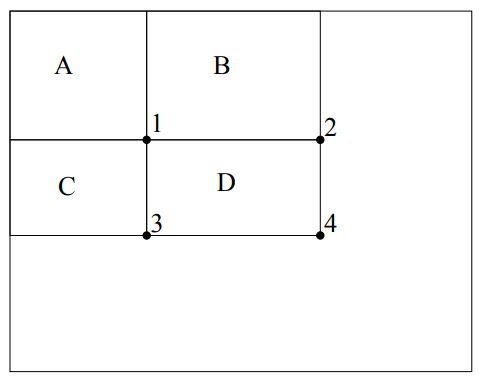
\includegraphics[width=.50\textwidth]{integralImage.png}
  \caption{The sum of the pixels within rectangle  can be
computed with four array references. The value of the integral image at location $1$ is the sum of the pixels in rectangle $A$. The value at location 2 is $A+B$, at location 3 is $A+C$,
and at location 4 is $A+B+C+D$ . The sum within $D$ can
be computed as $4+1-(2+3)$ \cite{Viola01rapidobject}}
  \label{fig:integralImage}
\end{figure}
The second thing that made calculations in the Viola-Jones algorithm so efficient is the use of simple rectangle features.
These features can be calculated very fast on the introduced integral images.
Examples of these rectangle features can be seen in Figure \ref{fig:simpleFeatures}.
\begin{figure}
  \centering
  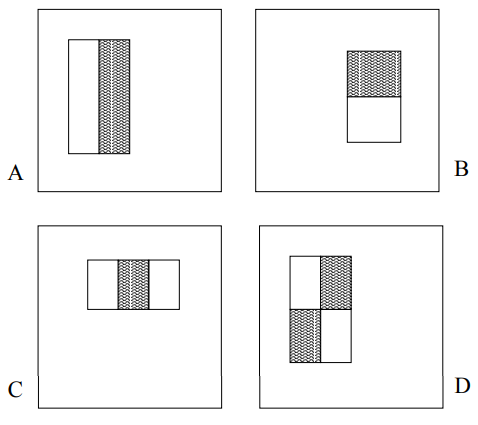
\includegraphics[width=.60\textwidth]{simpleFeatures.png}
  \caption{Example rectangle features shown relative to the
enclosing detection window. The sum of the pixels which
lie within the white rectangles are subtracted from the sum
of pixels in the grey rectangles. Two-rectangle features are
shown in (A) and (B). Figure (C) shows a three-rectangle
feature, and (D) a four-rectangle feature. \cite{Viola01rapidobject}}
  \label{fig:simpleFeatures}
\end{figure}
To learn a small number of important features AdaBoost\cite{FREUND1997119} is used. AdaBoost takes a bunch of weak classifiers and combines their results to a strong classifier.
Another features that was implemented is that the weak classifiers are calculated on subwindows of the original image.
The subwindows refer to a Region Of Interest(ROI).
The classification process works in multiple stages where first the features that have the lowest error rate will be used, while even weaker features come later. 
This so-called \emph{Attentional Cascade} makes it possible to make decisions even in earlier stages which accelerates computation time by a lot.
Although the detection cascade has 38 stages only 10 are used in average.
The Viola-Jones algorithm or variations of it are still used in a wide variety of applications, although classifiers using Convolutional Neural Networks(CNNs)(see Section \ref{ssec:convNets}) have shown to perform better.
Face detection with CNNs are more robust to the alignment of the face in the image. 
While Viola-Jones works very good for frontal faces CNNs can generalize better to also classify non-frontal faces.
Although the CNN approach is more robust it is only possible to run it in realtime on a GPU. This is because neural networks scale very good on GPUs but can be very slow an a CPU for bigger models.
To understand how neural networks work see Section \ref{sec:DeepLearning}.

\subsection{Object tracking}\label{ssec:objectTracking}
%What is it in general
Object tracking is a technique from the field of Image Processing. 
Object tracking became more relevant with the increasing amount of surveillance cameras.
Therefore the research interest in object tracking raised and in the recent years very robust algorithms were developed for object tracking. 
Very important aspects are the online capability as well as scale and translation independence. 
With the MOSSE tracker introduced in 2010 by Bolme et al. in \cite{BolmVisu2010} a robust translation independent approach was presented. In 2014 this approach was enhanced with scale independence by Danelljan et al. in \cite{Danelljan2014}. This approach was implemented in dlib \cite{Dlib} in 2015.
In the following the algorithm will be described.

%Corellation Filters
Correlation based tracking techniques use a filters to model the appearance of the tracking object. These correlation filters indicate how much a parts of an image $f$ correlate with the filter $h$.
The resulting output $g$ is of the same size as $f$ and has peaks in areas, that correlate most with the filter.
In figure \ref{fig:filtersApplied} an example of the application of different filters is given. It is obvious that for the purpose of tracking one of the correlation filters, namely Average of
Synthetic Exact Filters (ASEF)\cite{BolmAver2009}, Unconstrained Minimum
Average Correlation Energy (UMACE)\cite{Savvides2003}, and Minimum
Output Sum of Squared Error (MOSSE)\cite{BolmVisu2010}, suit better than the naive approach since they produce more compact peaks.

\begin{figure}
  \centering
  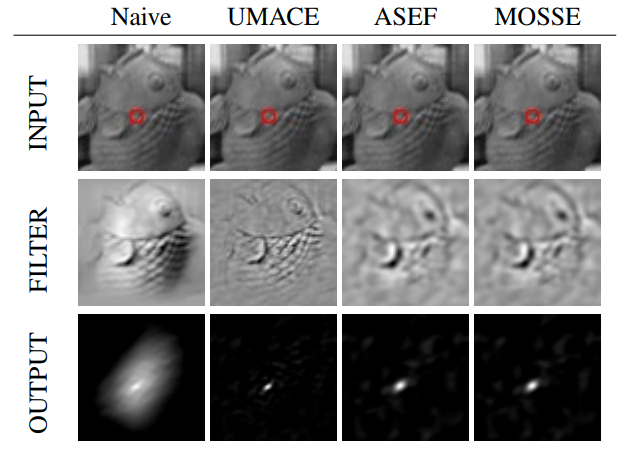
\includegraphics[width=.75\textwidth]{filtersApplied.png}
  \caption{Example of the application of different filters to a sample.  The three correlation
filters produce peaks that are much more compact than the
one produced by the Naive filter. \cite{BolmVisu2010}}
  \label{fig:filtersApplied}
\end{figure}

To track an object the filter $h_0$ is calculated from the first frame $f_0$ given a manually selected position window $p_0$ with the object of interest in center.
In the following frame $f_1$ the filter $h_0$ is applied to a search window. 
The search window is some kind of heuristic assuming the object can only move a limited distance between frames. 
In the resulting output $g_1$, the maximum value corresponds to the position the object moved. 
From this point on the filter $h_n$ is retrained dynamically with the position window $p_n$ of the object in the frame $f_n$.

To reduce computation time the filter is applied in the Fourier domain, since following the Convolution Theorem correlation becomes a element-wise multiplication in the Fourier domain. This results in

\begin{equation}
G = F \odot H^{*}
\end{equation}
where $G$, $F$, $H$ are the output, the input image and the filter in the Fourier domain respectively.
The $\odot$ operator denotes the element-wise multiplication and the $*$ indicates the complex conjugate.
$F = \mathcal{F}(f)$ and $H = \mathcal{F}(h)$ can be calculated with the Fast Fourier Transform (FFT)\cite{Nume2007}
while $g = \mathcal{F}^{-1}(G)$ can be calculated with the inverse FFT. 

While ASEF is averaging over "exact filters" to calculate the resulting filter, MOSSE is calculating the filter by minimizing the Sum of Squared Error (SSE) between the \emph{actual} and \emph{desired} output.
Since the training is conducted in Fourier domain a filter for a given image and output can be calculated element-wise as follows:
\begin{equation}\label{eq:filterSSE}
H^{*}_i = \frac{G_i}{F_i}
\end{equation}
To find a closed form for a filter that fits all given training images SSE is applied to Equation \ref{eq:filterSSE}, resulting in 
\begin{equation}\label{eq:minimize}
\min_{H^*} \sum_{i} |F_i \odot H^* - G_i|^2 
\end{equation}
Bolme et al. derive Equation \ref{eq:minimize} to the closed form 
\begin{equation}\label{eq:MOSSEFilter}
H^* = \frac{\sum_i G_i \odot F^*_i}{\sum_i F_i \odot F^*_i}
\end{equation}
For the initialization of the filter random small affine transformations are applied 
to the tracking window of the first frame. The resulting  perturbations $f_i$ and correspondingly generated outputs $g_i$ are used in Equation \ref{eq:MOSSEFilter} to calculate the initial filter $h_0$. From there on, as mentioned earlier, the online update is applied. Bolme et al. use a running average for the MOSSE filter to update as follows:
\begin{equation}
H^*_i = \frac{A_i}{B_i}
\end{equation}
\begin{equation}
A_i = \eta G_i \odot F^*_i + (1-\eta)A_{i-1}
\end{equation}
\begin{equation}
B_i = \eta F_i \odot F^*_i + (1-\eta)B_{i-1}
\end{equation}
$\eta$ denotes the learning rate, which puts more weight on recent frames and decays the influence of older frames exponentially over time.
%Failure detection
To detect tracking failures or occlusion the Peak to Sidelobe Ratio (PSR) is used. The PSR is a simple measurement of peak strength, which evaluates the peak from the correlation filter in respect to the noise. 
The PSR can be calculated with $\frac{g_{max} - \mu_{sl}}{\sigma_{sl}}$, where $g_{max}$ is the maximum of the correlation output $g$, $\mu_{sl}$ is the mean and $\sigma_{sl}$ is the standard deviation of the sidelobe. 
Whereas the sidelobe is considered to be the output $g$ without an 11 $\times$ 11 pixels area around the peak.
Bolme et al. showed in experiments that UMACE, ASEF and MOSSE filters produce a PSR between 20.0 and 60.0, if tracking is working properly. 
A PSR lower than 7.0 is a strong indicator, that the object is occluded or the tracking failed.
As mentioned earlier the Naive implementation produces peaks not as compact as the other filters, which results in a PSR ranging between 3.0 and 10.0. For the Naive implementation the PSR does not correlate to the tracking quality and therefore no conclusion can be drawn from the PSR.

%Evaluation
Bolme et al. evaluated the MOSSE filter in comparison to the UMACE, ASEF and the naive filter implementation on seven commonly used and freely available test videos from \url{http://www.cs.toronto.edu/\textasciitilde dross/ivt/}.
The results presented in Figure \ref{fig:eval} show that the MOSSE filter outperforms the other approaches in nearly every situation. %\cite{BolmVisu2010} 

\begin{figure}
\centering
  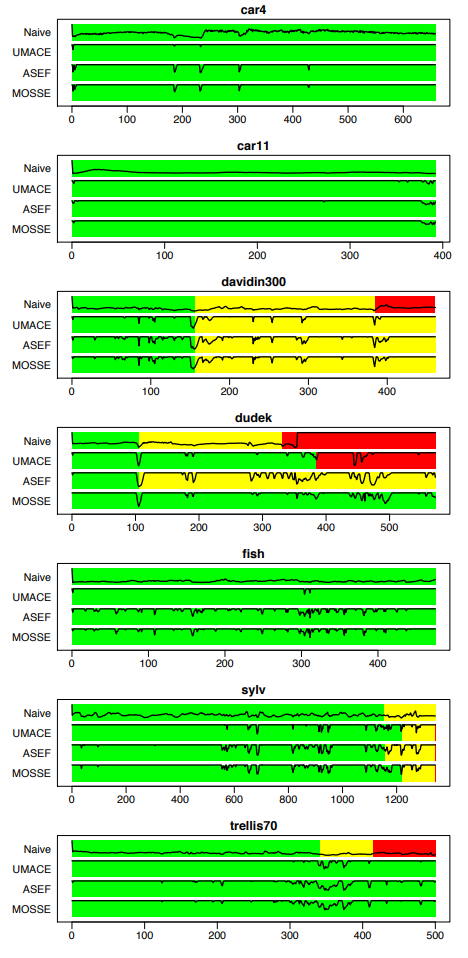
\includegraphics[width=.75\textwidth]{eval.png}
  \caption{This figure shows the performance of the filter based
trackers on all seven of the video sequences. Each output video
was hand annotated where Green indicates a good track, Yellow
indicates the track drifted off center, and Red indicates tracking
failure. The black lines shows PSR that was clipped to the range
[0,20] and indicates the quality of the track for each frame of the
video. \cite{BolmVisu2010}}
  \label{fig:eval}
\end{figure}

%Scale independency from Danelljan et al.
As mentioned earlier the MOSSE filter approach is extended by Danelljan et al. in \cite{Danelljan2014} with a scale estimation to increase robustness in situations where large scale variations appear.Therefore a separate scale correlation filter is used.
This filter is updated with a training example $f$, which is constructed from features, that use different patch sizes centered around the target.
This filter is applied to the target location calculated by the translation filter.
This technique saves some computation time and is possible because the difference in scale between to successive frames is normally smaller than the difference in translation. This enables the approach to accurately and computationally efficient estimate translation and scale of a tracking object in a video sequence.




% Learning algorithms
\section{Learning Algorithms}\label{sec:learningAlgorithms}
This section describes all the theoretical parts of a Learning Algorithm. Starting from the data and how to handle it going to different approaches to make sense out of data ending in specific learning algorithms.
\subsection{Data}\label{ssec:dataTheory}
Data Scientist are coming up with new algorithms to solve specific problems nearly everyday and they lead to astonishing results in the field of Natural Language Processing and Image Classification.
New Algorithms and better Hardware brought fields like Optical Character Recognition, Automatic Speech Recognition and Image Classification to a near-human level. 
With this new achievements and a growing basis of publicly available datasets people tend to forget that the foundation of learning is the data. Exactly these huge publicly available datasets, like ImageNet\cite{ImageNet} with more than 14 million images in over 20 thousand categories, are the reason why Data Scientist could develop new algorithms and effectively use Deep Learning.


The fanciest algorithms with cutting edge hardware will not learn the desired relation if the data is corrupted or simply not suited for the task.
So when it comes to developing a learning algorithm it is important to know what the goal is and what relation the data can provide.
For a lot of projects publicly available datasets offer a good starting point to either use the data directly or extract a new dataset for a specif task from it. 
\url{https://www.kaggle.com/datasets} offers a wide range of datasets for all kinds of applications.

After carefully selecting the data it is important to split the data in three different parts. 
Most of the publicly available datasets are already divided in \emph{training data}, \emph{validation data} and \emph{test data} and newly constructed datasets should be divided in the same categories.
With these three subsets it is possible to effectively evaluate an algorithm.
This brings the advantage of comparability for different algorithms on the same problem.
The subsets have the following functions:

\begin{description}
\item[Training Data]\hfill \\
The training data is the biggest subset of the dataset and takes normally around 70-80\% of the data. This data is used to train the learning algorithm.
\item[Validation Data]\hfill \\ 
The validation data is used to validate the the algorithm while searching for suitable hyper parameters(see \ref{ssec:hyperP}) and prevent overfitting(see section \ref{ssec:overfitting}).
The validation data normally takes around 10-15\% of the data.
\item[Test Data]\hfill \\ 
The test data is only used once in the very end to evaluate the algorithm.
The test data normally takes around 10-15\% of the data.
\end{description}

\begin{figure}
\centering
  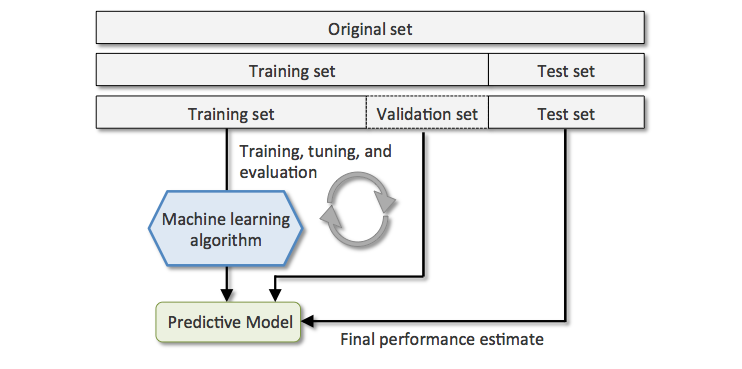
\includegraphics[width=.75\textwidth]{training_validation_test.png}
  \caption{Dividing and using a dataset correctly \cite{DataSplit}}
  \label{fig:dataSplit}
\end{figure}


One could ask if the test data evaluates the algorithm what is the validation data for?
While searching for a good model for the problem the hyper parameters will be adjusted to get the best results on the validation data. 
The process of searching for the perfect hyper parameters can be viewed as \emph{learning} only that it is not the algorithm that learns the best parameters to satisfy the training data, but the Data Scientist that learns the best hyper parameters to satisfy the validation data. This process is as well prune to overfitting.
This also explains why the test data can only be used once.
Changing anything about the model because of the performance of the test data, the assessment of generalizability will be flawed.

In terms of constructing a dataset three aspects should be considered very carefully.

\begin{description}
\item[Representativeness of the data]\hfill \\
It is important that training, validation and test data represent the whole dataset. 
In a classification task with 10 classes, where the training data holds only samples from the first 8 classes, while validation data only holds class 9 and the test data only holds samples of class 10, the algorithm can obviously never perform well on the validation or test data. 
To prevent such behavior the dataset should be randomly shuffled.
\item[Redundancy of the data]\hfill \\ 
Redundant data happens a lot, that is basically no problem. 
The problem comes up, when the sample ends up in training data and validation or test data.
When that happens evaluation(validation or test) is actually happening on some part of the training data, which flaw the assessment of generalizability.
\item[Time dependency of the data]\hfill \\ 
If the task is to predict the future from the past it is important not to shuffle the dataset randomly, because otherwise the model will be trained on future data and evaluated on past data which is the opposite of what was the goal.
\end{description}

\subsection{Preprocessing}\label{ssec:preprocessing}
After choosing the right data for the desired task and dividing it into training, validation and test data often another step is necessary before the training can start.
This step is called preprocessing and describes the transformation of the data into a shape, that fits the selected algorithm best.
These transformations can be arbitrary but the following transformations are common:
\subsubsection{Data Cleaning}
Data cleaning deals with the detection and correction(or removal) of duplicates, corrupted samples and outliers. 
If corrupted samples get into the learning process, it can influence the results a lot. For example if a feature is out of its known range, it can be rejected or corrected before even considered in the training process.
\subsubsection{Normalization}\label{ssec:normalization}
A lot of the learning algorithms have problems if features have a great difference in scale between each other. 
With this in mind it makes sense to normalize the features to a common range. 
It is common practice to normalize the features to a mean of 0 and a standard deviation of 1. Some algorithms are expecting values in this shape or at least working optimal with those. If gradient descent is used to optimize the model parameters this helps to keep the gradient of the loss function at small values.\cite{CholDeep2018}

\subsubsection{Feature Extraction}\label{ssec:featureExtracion}
A dataset consists of samples which describe a observation.
These samples consist of features and labels (if we consider supervised learning). Features are normally denoted as 
$\mathbf{x} = \left\langle x_{0}, x_{1}, \cdots , x_{n-1}, x_{n} \right\rangle$ while labels are denoted as $\mathbf{y} = \left\langle y_{0}, y_{1}, \cdots , y_{m-1}, y_{m} \right\rangle$
Since the general goal of learning algorithms is to find a mapping between $\mathbf{x}$ and $\mathbf{y}$ it makes sense to take a closer look to the features.
Features can be of very different shape, but the more compact the information is represented the easier is it for the learning algorithm to find a mapping.
In Figure \ref{fig:featureClock} an example of the same information in different shapes is given.  
\begin{figure}
\centering
  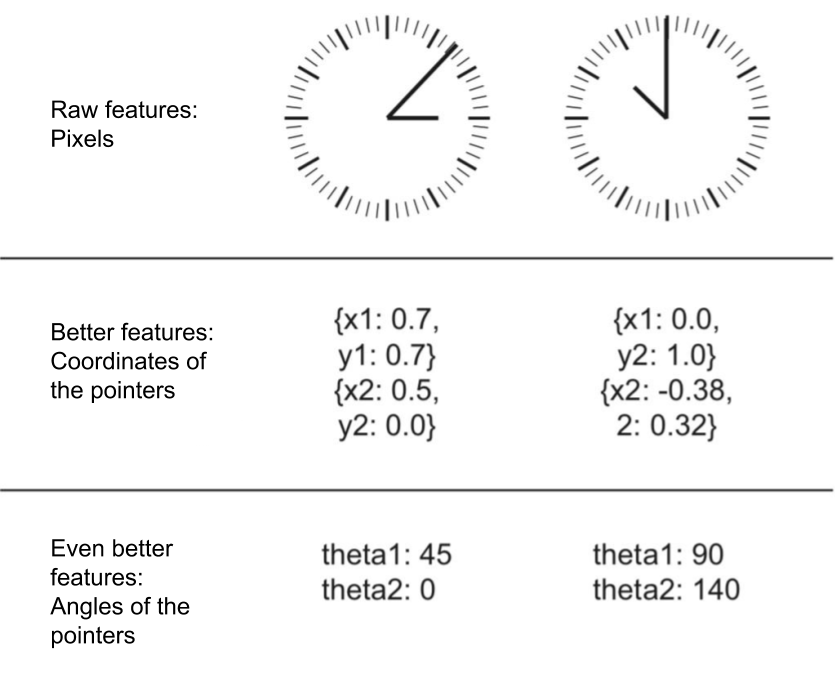
\includegraphics[width=.75\textwidth]{featureClock.png}
  \caption{Different types of features for the same problem \cite{CholDeep2018}}
  \label{fig:featureClock}
\end{figure}
This example shows very nice how feature extraction can decrease the input shape and size by a lot, which makes learning essentially easier. 
Assuming the image of the clock is $64 \times 64$ pixels the input would be a two-dimensional array with 4096 values.
Learn a mapping between this input values and the time as output value is a relatively complex task that would need a CNN to be trained. 
So using the raw features would lead to a significant computational effort.
In contrast extracting the coordinates of the tip of the pointer would end up in an 1-dimensional input shape with four values. 
Learning the mapping between the coordinates and the time is essentially easier.
Taking it even further changing the coordinate system from a Cartesian coordinate system to a polar coordinate system the input can be reduced to two values.
And for that learning wouldn't be necessary. Rounding of the values and putting the corresponding time in a dictionary would be enough.

Domain knowledge can be very helpful to make learning easier for the algorithm.
Before Deep Learning became really applicable feature extraction was a big and important part in data science.
Good features decided about the quality of shallow learning approaches.
In Deep Learning the hypothesis space is essentially bigger which makes it possible to learn those features on the fly.
For learning these features a lot of data is needed, so if only little data is available feature extraction is still important.
It is important to have in mind, that the features in Deep Learning are learned automatically, so it makes sense to verify the learned features. 

For example if a CNN should classify if a male or female is in a picture and the dataset consists of images from males and females, but females are always captured in front of a white background and males are always captured in front of a black background the CNN will most certainly learn that and will perform poorly on images with blue background.
Humans wouldn't take the background in consideration because they already know the domain of the problem.
The CNN doesn't know anything, so everything will be considered.

\subsection{Categories of Learning}
In general learning can be viewed as finding a mapping from an input $\mathbf{x}$ and an output $\mathbf{y}$.
Figure \ref{fig:learning} shows a schematic overview on how to come from data to a hypothesis that can make predictions after training.

\begin{figure}
\centering
  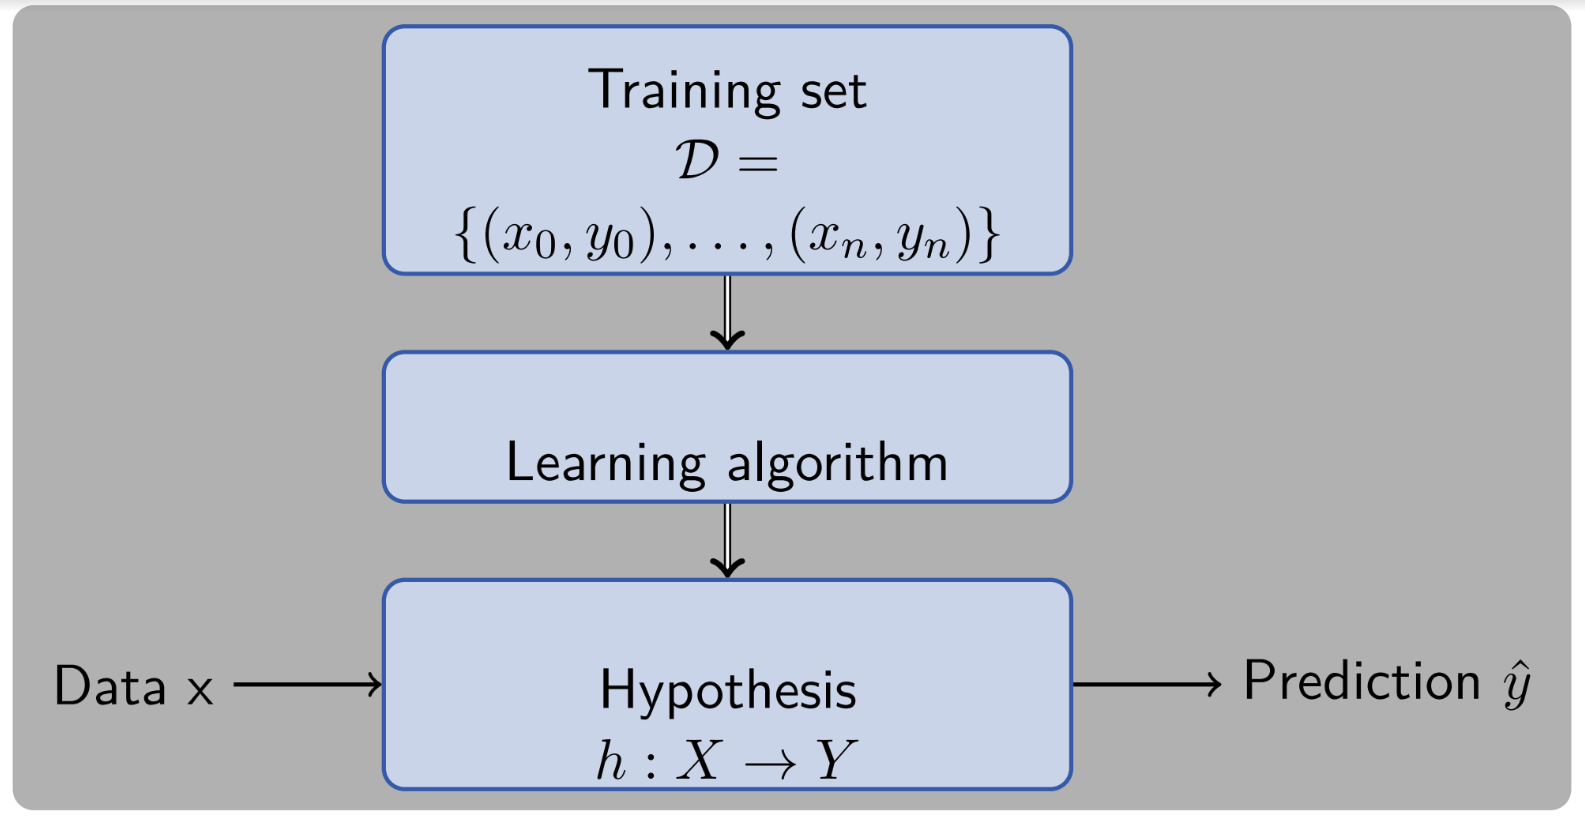
\includegraphics[width=.75\textwidth]{learning.png}
  \caption{The overall structure of learning.\cite{LVDFKI}}
  \label{fig:learning}
\end{figure}

Learning can be divided into four different categories.
At some point they can overlap a little but most of the time problems can be classified in one of the following categories.

\subsubsection{Supervised Learning}
In Supervised Learning the learning algorithm is fed with labeled data and the goal is to learn a hypothesis $h$ that maps the input $\mathbf{x}$ to the output $\mathbf{y}$.
As shown in Figure \ref{fig:learning} the Training set $\mathcal{D}$ consists of input values $x_i$ and their corresponding output value $y_i$. These labels are often also called the \emph{ground truth} because this is the information, that is true and should be learned.
This is given to a learning algorithm, which calculates a hypothesis(this is often also called a model) of the data, which is able to predict an output $\hat{y}$ for a given input $x$.

There are basically two types of Supervised Learning.
If the output data is in the discrete domain the task is called \emph{Classification}.
A very easy example would be the classification of handwritten digits, where the input would be a grid of pixels(an image) and the output would be an integer from 0 to 9. 
(Example from the MNIST dataset for handwritten digits\cite{YannGrad1998} available under \url{http://yann.lecun.com/exdb/mnist/}) 

In contrast if the output data is in the continuous domain the task is called \emph{Regression}.
An easy example for regression would be to predict the price of a house by attributes like \texttt{per capita crime rate by town}, \texttt{Average number of rooms per dwelling}, \texttt{Index of accessibility to radial highways} and many more. 
(Example from the Boston Housing dataset\cite{Harrison78} available under \url{https://www.kaggle.com/c/boston-housing}) 

Supervised Learning is by far the category with the most applications.
This is because it is relatively easy to evaluate the accuracy of the developed learning algorithm, because the ground truth is available to apply several metrics(see section \ref{ssec:lossFunc}) to the results.

\subsubsection{Unsupervised Learning}
Unsupervised Learning describes a category of learning where the ground truth is not known. 
For Unsupervised Learning the Training Data $\mathcal{D}$ shown in figure \ref{fig:learning} would lack the labels $y_0$ to $y_n$.
With no ground truth available the learning algorithm can only find previously unknown patterns in the data.

\emph{Clustering aims at partitioning $n$ observations into $k$ clusters.
Observations that are assigned to the same cluster should be more
“similar” than those belonging to different clusters.}\cite{LVDFKI}

Clustering helps Data Scientist to to understand the data better and to discover existing correlations in it.
Sometimes clustering is an important first step towards a Supervised Learning task. 
As stated before Unsupervised Learning is harder to evaluate because there is no ground truth to evaluate the results on.
Figure \ref{fig:clustering} shows some examples of clustering algorithms and how they perform in different scenarios.

\begin{figure}
\centering
  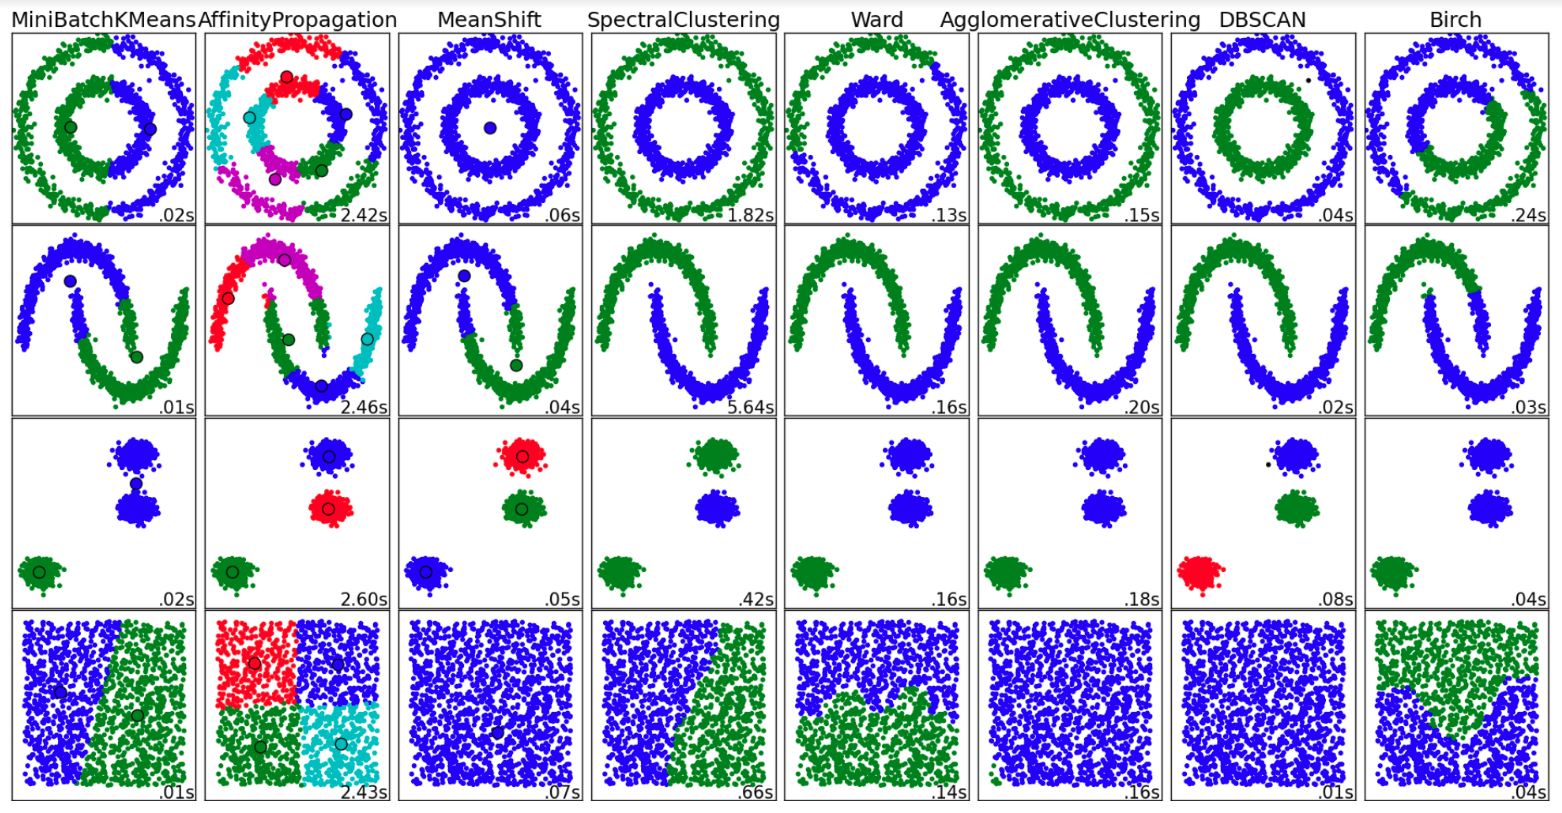
\includegraphics[width=.75\textwidth]{clustering.png}
  \caption{clustering algorithms and how they perform in different scenarios.\cite{LVDFKI}}
  \label{fig:clustering}
\end{figure}

\emph{Dimension Reduction} is another technique that can be performed unsupervised.
The goal of Dimension Reduction is to reduce the dimensionality of the input data.
An example of Dimension Reduction would be the Principal Component Analysis, which finds the features with the highest variation in the data. The highest variation is closely related to the meaningfulness of the features. 
If specific features have no or nearly no meaningfulness they can be dropped and therefore reduce the dimensionality of the data.



\subsubsection{Self-supervised Learning}
Self-supervised Learning is more or less a sub category of Supervised Learning, where labels are automatically extracted from unlabeled data, to then start a supervised learning process. 
A simple example for Self-supervised Learning would be to predict the next frame of a video sequence or the next word of a sequence of words.
Here no labels are available but sequences have the neat ability, that they have implicit output values when it comes to predicting the next element of a sequence.
For the example with sequences of words it is possible to just have a bunch of phrases and extract labeled sequences by always taking $x$ words as input and the $x+1$ word as the label.


\subsubsection{Reinforcement Learning}
Another very interesting category of learning is \emph{Reinforcement Learning}, where an \emph{Agent} learns to conduct different \emph{Actions} in an \emph{Environment} to maximize a \emph{Reward}.
An Example would be a learning Agent that takes the screen of a video game as the input and learns to perform the best actions to gain the most points.
This category gained a lot of attention lately through the astonishing performance of AlphaGo \cite{AlphaGo} to be the first AI, that won against a human champion.


\section{Deep Learning}\label{sec:DeepLearning}
As described in Section \ref{sec:approach} the VVAD is implemented using a LSTM-FCN, which is a neural network containing a convolutional part to model the spatial features and a recurrent part to model the temporal features. 
In this section, all theoretical aspects of an LSTM-FCN are explained.
\subsection{Artificial Neural Network(ANN)}
An Artificial Neural Network can be described as the attempt to model the human brain in a computer. As the human brain is very complex and research in this field is not certain about every aspect and a large part is still completely unexplored, the connection between an ANN and the human brain is very loose and only models the parts, that scientists are very certain about. 
This is the fact that the brain consists out of around 100 billion of neurons interconnected in a complex network structure \cite{Herculano09}.
The "wire" that connects neurons is called axon and is in fact acting like a wire that transmits  small potentials  between the neurons.
The axons can have different conductivity depending on how frequently they are used.
This is very important because it is one of the ingredients how human can learn. 
This concept is called \emph{weights} in an ANN. How \emph{weights} are implemented in an ANN and how that impacts learning will be discussed later.
One neuron can have multiple incoming and one outgoing axons. 
Without mentioning all the biochemical processes happening at this point, one can simplify and say all incoming axons merge into the axon hillock where, if a certain threshold is reached the neuron invokes a potential itself ("fires").
The merging of axons is a summation of the transported potential, where the potential can be excitatory (having a positive influence on the sum) or inhibitory (having a negative influence on the sum). In an ANN excitatory potentials would be positive \emph{weights} while inhibitory potentials would be negative \emph{weights}.
\cite{BGDFKI}
So one neuron can be seen as some kind of a gate which decides if the sum of some incoming signals is worth to fire an outgoing signal.
And the whole network of neurons can be seen as sieve that allows only specific paths for the potentials to go through the network. 
The well known experiment called \emph{Pavlov's Dog} is a good example to show how these paths work.

\paragraph{Pavlov's Dog:}
A Dog is presented two different stimuli. As presented in Figure \ref{fig:pavlov} these are a unconditioned stimulus(food) and a neutral stimulus(bell ringing). The unconditioned stimulus produces a unconditioned response, which is salivation in the case of Pavlov's dog. The goal in the experiment is to show that it is possible to condition the dog to show the same response on the bell ringing.

\begin{figure}
\centering
  \includegraphics[width=.75\textwidth]{Classical_Conditioning_Diagram.png}
  \caption{Classical Conditioning Diagram \cite{pavlovsDog}}
  \label{fig:pavlov}
\end{figure}

\paragraph{} %pseudo end of the paragraph before
To understand how the dog \emph{learns} to salivate on the ringing of the bell the analogy of the paths is used.
The smell of the food activates some nerve cells in the dog's nose. The invoked potentials are forwarded to the brain, where the \emph{sieve} decides which action is mapped to the incoming signal. The signal takes a path over several neurons to end up in a place which activates the salivation. 
This path was already there and is probably one of the \emph{preprogrammed} paths a dog was born with. 
These \emph{preprogrammed} paths are learned evolutionary.
If the dog is presented the neutral stimulus salivation will not be activated because there is no path between the nerve cells from the ears and the neurons that activate the salivation.
As the dog is presented both stimuli the brain gets the described two inputs.
Another very important mechanism for learning takes effect here.
If something "good" is happening all recently active axons will be strengthened which results in a higher conductivity.
If something "bad" is happening the effect is flipped.
ANNs try to reproduce this mechanism mathematically by a procedure called backpropagation(see section \ref{ssec:backProp}).
The brain has very complex mechanisms to decide what is "good" and "bad". This is not relevant for the example and will not be discussed any further. 
In the example the assumption holds that food is something "good" and therefore all recently active axons will be strengthened. 
This means that also all the axons corresponding to the bell ringing will be strengthened. 
If the axons' conductivity is higher a higher potential can be transmitted and therefore reach a higher summed potential in other neurons. If the potential is higher than a certain threshold this neuron will fire. 
This means the path from the neurons corresponding to the bell ringing will enlarge every time both stimuli are presented at the same time.
After a while this will eventually lead to the development of a path between the bell ringing and the salivation neurons.
This explains, why the dog \emph{learned} to salivate on bell ringing.
Knowing this it makes also sense that the effect will vanish if the bell ringing is presented too often without the reward of the food, because being tricked is considered as something "bad" by the brain.
In the human brain neurons can be connected very arbitrary, while modern ANNs normally structure their artificial neurons in so called \emph{Layers}.
Figure \ref{fig:3layers} shows a ANN with three layers.
Each layer consists of a number of artificial neurons that are connected to the previous and subsequent layer.

\begin{figure}
\centering
  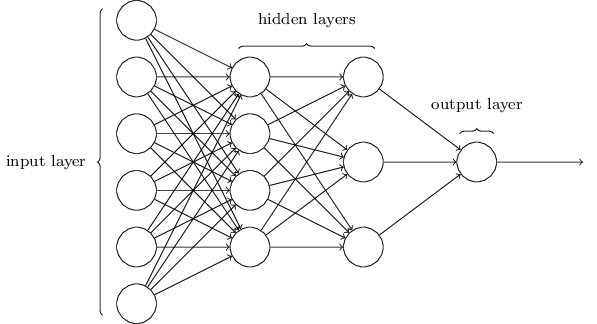
\includegraphics[width=.75\textwidth]{3layers.png}
  \caption{A neural network with one input layer, two hidden layers and an output layer.\cite{Nielsen2015}}
  \label{fig:3layers}
\end{figure}

\subsection{Artificial Neuron}\label{artificialNeuron}
The smallest element of an ANN is the artificial neuron.
The modern artificial neurons are inspired by the concept of a perceptron, which was developed by Frank Rosenblatt in the 1960s \cite{rosenblatt1962principles}.
The perceptron is the first approach to model a neuron in a computer.
A perceptron can have multiple inputs and one output, just like a neuron in the human brain.
Figure \ref{fig:perceptron} shows an example of a perceptron with the three inputs $x_1, x_2, x_3$.

\begin{figure}
\centering
  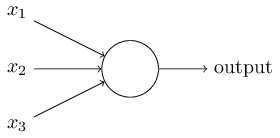
\includegraphics[width=.75\textwidth]{perceptron.png}
  \caption{A perceptron with input $x_1, x_2, x_3$ \cite{Nielsen2015}}
  \label{fig:perceptron}
\end{figure}

To calculate the output Rosenblatt introduced the concept of \emph{weights}, which describe how important a specific input is for the output.
The classical perceptron produces a binary output, which is calculated using equation \ref{eq:perceptron}.
\begin{equation}\label{eq:perceptron}
output = \left\{\begin{matrix}
0 & \mathrm{if} \sum _j w_j  x_j\leq \mathrm{threshold}\\ 
1 & \mathrm{if} \sum _j w_j  x_j>  \mathrm{threshold}
\end{matrix}\right.
\end{equation}
This equation is the \emph{activation function} of the perceptron. 
It basically decides whether the perceptron fires or not.
If equation \ref{eq:perceptron} is applied with the dot product of the vector $w = \left\langle w_1, w_2, ..., w_n  \right\rangle$ for the weights and $x = \left\langle x_1, x_2, ..., x_n  \right\rangle$ for the inputs, it is possible to move the threshold to the other side of the inequality. Furthermore the threshold is replaced by an new variable called \emph{bias} in the following fashion: $b \equiv -\mathrm{threshold}$

This leads to equation \ref{eq:heaviside} which is basically the Heaviside step function

\begin{equation}\label{eq:heaviside}
output = \left\{\begin{matrix}
0 & \mathrm{if} \ w \cdot x + b\leq 0\\ 
1 & \mathrm{if} \ w \cdot x + b >  0
\end{matrix}\right.
\end{equation}

Rosenblatt proved that a single perceptron can implement the logic operation \texttt{NAND} which is a basic logic operation. 
This means all other logic operations can be build using a \texttt{NAND}. 
This is shown in the following example:

Figure \ref{fig:NAND} shows a perceptron with two inputs and the corresponding \emph{weights} of $-2$ and a \emph{bias} of 3.
\begin{figure}
\centering
  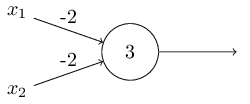
\includegraphics[width=.75\textwidth]{NAND.png}
  \caption{The perceptron implements a logic \texttt{NAND} gate \cite{Nielsen2015}}
  \label{fig:NAND}
\end{figure}
Giving the input $x_1=0;x_2=0$ the perceptron will output $1$, hence $(-2) \cdot 0 + (-2) \cdot 0 + 3 = 3$ is positive. 
Doing the same calculation for the input where either one of the inputs is $0$ and the other is $1$ shows the same output but if both input values are $1$ the formula produces an output of $0$, since $(-2) \cdot 1 + (-2) \cdot 1 + 3 = -1$ is negative.
With the \texttt{NAND} gate it is for example possible to build the bitwise addition.
Figure \ref{fig:NANDADD} shows how multiple perceptrons can be linked to a network to implement the addition of two input bits with a carry bit which depicts if both inputs are $1$ which would lead to a resulting sum of $2$.
$2$ is not mappable in a single bit representation, therefore the carry bit shows the overflow.

\begin{figure}
\centering
  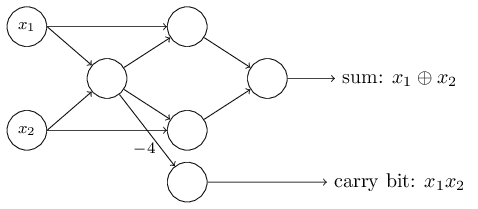
\includegraphics[width=.75\textwidth]{NANDADD.png}
  \caption{A network of perceptrons building the bitwise addition of two inputs. All weights are -2 and all biases are 3 as shown in Figure \ref{fig:NAND}. The -4 means that the input is the same for $x_1$ and $x_2$ of that perceptron \cite{Nielsen2015}}
  \label{fig:NANDADD}
\end{figure}

This already shows that networks of perceptrons are quite powerful but the problem is, that in the given example all weights were given and the goal of \emph{Learning} is to abstract these out of given samples.
There are two main problems when it comes to learning the weights of a classical perceptron.
\begin{itemize}
\item[1.] The state of the art way to train neural networks is by using gradient descent (see Section \ref{ssec:gradientDescent}) with backpropagation (see Section \ref{ssec:backProp}).
Backpropagation requires the activation functions of the artificial neurons to be differentiable. 
Hence the Heaviside step function used by the classical perceptron is not differentiable at $x = 0$ and has a gradient of $0$ anywhere else, the gradient descent method won't work here.
\item[2.] Mathematically speaking, \emph{learning} the weights for a neural network is an optimization problem. 
The goal here is to find the weights that produce the smallest error on the output.
Optimizing in this case is only possible if small changes in the weights cause only small changes in the resulting error.
Since the Heaviside step function can only produce $0$ and $1$ as output, it does not fulfill this requirement.
\end{itemize}

\subsection{Activation Function}
As described earlier the \emph{activation function} is a function that decides whether an artificial neuron fires or not. 
Since the classical perceptron does not fulfill the requirements to be used with backpropagation and gradient descent new activation functions needed to be developed to make neural networks a solvable optimization problem.
Additionally to the requirements that the activation function needs to be differentiable and small changes in the weights should have a small impact on the output, non-linearity is a very important requirement.
A combination of layers of artificial neurons with linear activation functions can only lead to a overall linear function to model the data.
To model non-linearity in data it is important to have non-linear activation functions.
Following three of the most used and well known activation functions will be presented.
\paragraph{Sigmoid Function:}
The sigmoid function, sometimes also known as the logistic function, gives an output between $0$ and $1$. 
It is defined by by equation \ref{eq:sigmoid} and Figure \ref{fig:sigmoid} shows the course of the resulting curve.
\begin{equation}\label{eq:sigmoid}
sigmoid(x) = \frac{1}{1 + e^{-x}}
\end{equation}
\begin{figure}
\centering
  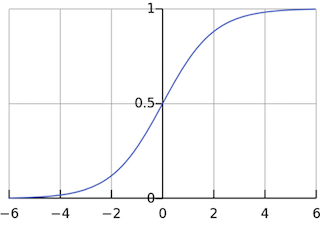
\includegraphics[width=.50\textwidth]{sigmoid.png}
  \caption{The shape of the sigmoid function \cite{Chris2017}}
  \label{fig:sigmoid}
\end{figure}
The sigmoid function fulfills all the requirements to be used with gradient descent and backpropagation. 
It is differentiable as there are no hard edges in the curve and it shows small and steady changes for small changes in the input and it is obviously non-linear. Despite all these positive aspects it has one major drawback.
The sigmoid function is at risk of facing the problem of the \emph{vanishing gradient}. The vanishing gradient will be discussed in a little more depth in Section \ref{ssec:backProp}, but the problem is very visible for very large positive or negative input values.
The output values for these input values are very close to either $0$ or $1$ but don't change a lot in this areas. 
This means the gradient is very small or even vanishes and this means gradient descent can no longer work to find the minimal error, which means there is no \emph{learning}.
This effect gets even stronger the more layers are stacked upon each other and can make the training of deep models very slow to impossible.

\paragraph{Tanh Function:}
The tanh function is very similar to the sigmoid function.
It is defined by Equation \ref{eq:tanh} and Figure \ref{fig:tanh} shows the course of the resulting curve.
\begin{equation}\label{eq:tanh}
tanh(x) = \frac{e^x - e^{-x}}{e^x + e^{-x}}
\end{equation}
\begin{figure}
\centering
  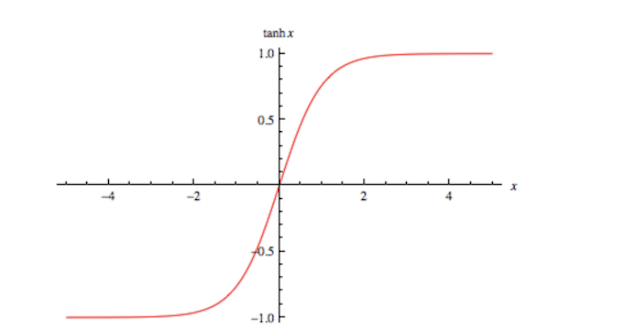
\includegraphics[width=.60\textwidth]{tanh.png}
  \caption{The shape of the tanh function \cite{Chris2017}}
  \label{fig:tanh}
\end{figure}
Figure \ref{fig:tanh} shows that sigmoid and tanh functions are very similar except that the tanh function maps the output to values between $-1$ and $1$.
Because of the close similarity the tanh function shares the same drawbacks as the sigmoid function.

\paragraph{ReLu (Rectified Linear Unit):}
The ReLu activation function is quite different to the sigmoid and tanh function. It is defined by Equation \ref{eq:relu} and Figure \ref{fig:relu} shows the course of the resulting curve.
\begin{equation}\label{eq:relu}
relu(x) = max(0, x)
\end{equation}
\begin{figure}
\centering
  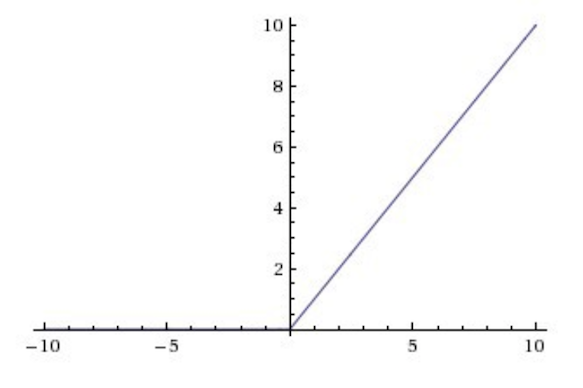
\includegraphics[width=.60\textwidth]{relu.png}
  \caption{The shape of the ReLu function \cite{Chris2017}}
  \label{fig:relu}
\end{figure}
On the first sight the ReLu looks very linear and intuitively one wouldn't expect it to perform very well.
As ReLu is computational very efficient and it is known to have no vanishing gradients Johnson et al. proposed to use the ReLu as the default non-linearity \cite{ConvNNs}.
Although the ReLu can handle the problem of \emph{vanishing gradients} it develops a new problem.
The \emph{dying ReLu} describes a phenomenon where a single artificial neuron will never be able to fire and therefore can be described as dead.
This happens when the activation value generated by an artificial neuron is $0$ during the forward pass over some iterations which causes it's weights to go to $0$ and it will never be able to fire again.

\subsection{Gradient Descent}\label{ssec:gradientDescent}
As mentioned earlier \emph{Learning} is basically an optimization process with the goal to find the parameters $\theta$ that minimize a loss(sometimes also referred to as cost) function $L(\theta)$(loss functions are explained in more depth in Section \ref{ssec:lossFunc}).
The gradient of the loss function is defined in equation \ref{eq:gradient} and \ref{eq:gradient_i}
\begin{equation} \label{eq:gradient}
g = \nabla_{\theta} L(\theta)
\end{equation}
\begin{equation} \label{eq:gradient_i}
g_i = \frac{\partial}{\partial\theta_{i}}  L(\theta)
\end{equation}
The gradient is basically the change in a function. 
Considering a linear regression model defined as 
\begin{equation}
y = \beta_0 + \beta_1 x_1
\end{equation}
the best values for $\beta_0$ and $\beta_1$ can be found using some x-y-points that should model the line (see Figure \ref{fig:points}), a loss function(in this case the mean squared error(MSE) is a good fit) and gradient descent as optimizer.
\begin{figure}
\centering
  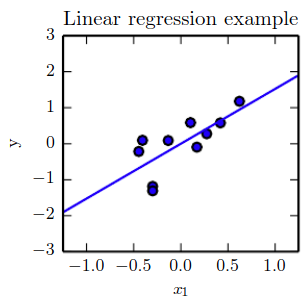
\includegraphics[width=.50\textwidth]{points.png}
  \caption{A linear regression problem, with a training set consisting of ten data points \cite{Goodfellow-et-al-2016}
}\label{fig:points}
\end{figure}
MSE will be discussed in detail in Section \ref{ssec:lossFunc} for now it is only important to know, that MSE maps the loss for the parameters $\beta_0$ and $\beta_1$ and the goal is to find its minimum.
Figure \ref{fig:gradientDescent} shows how the loss behaves plotted over $\beta_0$ and $\beta_1$.

\begin{figure}
\centering
  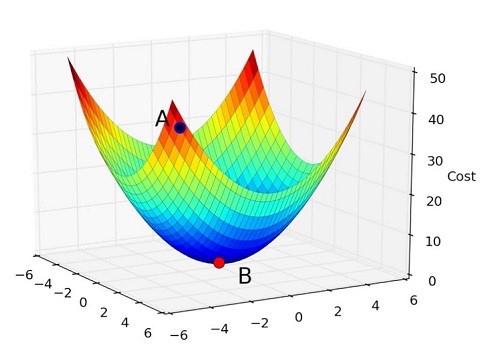
\includegraphics[width=.60\textwidth]{gradientDescent.jpeg}
  \caption{The goal for gradient descent is to go from a randomly initialized point A to the minimum in point B \cite{gradDescent}
}\label{fig:gradientDescent}
\end{figure}
The gradient descent is a iterative method, which only considers the gradient of a function and depending on the value of the gradient it will move the parameters towards the minimum.
Mathematically this can be formulated as 
\begin{equation}\label{eq:gradDescUpdate}
\theta_{n+1} = \theta_n - \alpha \nabla L(\hat{y}, y)
\end{equation}
$\hat{y} = y_{\theta_n}(\mathbf{x})$ is the prediction made from the model with the parameters $\theta_n$ \cite{ValdenegroToro2019DeepNN}.
The update for the parameters from equation \ref{eq:gradDescUpdate} can be computed for a predefined number of steps or until the change in the loss or the gradient stays under a predefined value for a predefined number of iterations.
$\alpha$ in equation \ref{eq:gradDescUpdate} is the \emph{Learning Rate}, which decides how much influence one update step has on the parameters.
In the given example of a linear regression model the parameters 
$\beta_0$ and $\beta_1$ would be optimized coming from point A and ending up in the minimum in point B.
Equation \ref{eq:gradDescUpdate} can be applied in the same way to deep neural networks. As the number of parameters for these deep neural networks (DNNs) is essentially bigger, the loss surface can not be plotted in a human-readable way. 
With a higher dimensionality of the parameters the hypotheses space will grow exponentially. This phenomena is known as the \emph{curse of dimensionality} which also explains why Deep Learning needs so much data to efficiently learn.
%influence of LearningRate and lossSurface
The success of gradient descent largely relies on the following two factors:
\paragraph{Learning Rate}
As mentioned earlier the \emph{Learning Rate} decides how much influence one update step has on the parameters. 
It is very important to set a good value here. If the Learning Rate is to big the optimization process can get very unstable and the minimum will not be reached due to overshooting. 
On the opposite if the Learning Rate is to small convergence can take too long as depicted in Figure \ref{fig:lr}.
\begin{figure}
\centering
  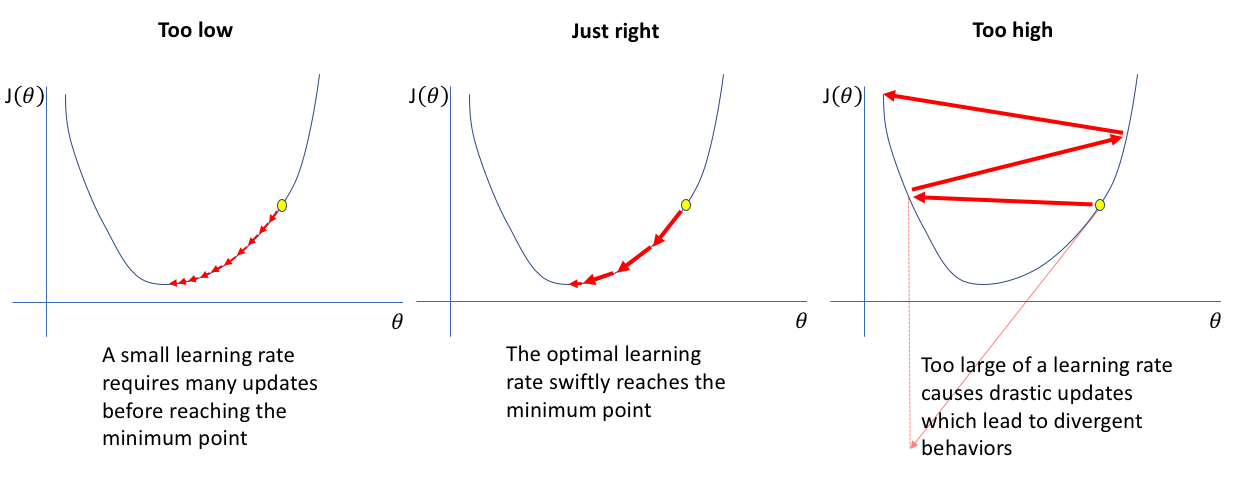
\includegraphics[width=\textwidth]{lr.png}
  \caption{Setting the correct learning rate is essential for good and fast convergence \cite{lr}
}\label{fig:lr}
\end{figure}
Typical values of the learning rate are $\alpha \in [0,1]$, and common starting values are $10^{-1}$ or  $10^{-2}$.\cite{ValdenegroToro2019DeepNN}. 
It is even common practice to change the Learning Rate during training. 
Common approaches are to
decrease the learning rate by a factor after a certain number of
iterations, or to decay the learning rate by a factor after each step. \cite{ValdenegroToro2019DeepNN}
\paragraph{Loss Surface}
Figure \ref{fig:gradientDescent} shows a very simple Loss Surface, for which it is imaginable easy to find the minimum but models more complex than the linear regression produce more complex loss surfaces. 
If the gradient in the loss surface gets to small or to big gradient descent is prone to the problem of vanishing / exploding gradient, because backpropagation in DNNs makes these values become more extreme.
The optimal loss surface is convex and has a smooth geometry.
In practice a non-convex loss function
is not a big problem, and many theoretical results show that the
local optima in deep neural networks are very similar and close
in terms of loss value. \cite{ValdenegroToro2019DeepNN}
\paragraph{} %pseudo end of the paragraph before
Gradient Descent comes in different variations.
The update rule given in equation \ref{eq:gradDescUpdate} is actually called Batch Gradient Descent and takes all training samples into account at once. 
This method basically takes the whole "batch" of training samples to do the update. 
This implicitly assumes that the whole dataset fits into memory. 
Recalling the curse of dimensionality this can lead to problems for more complex models which need a lot of data to train sufficient.
Furthermore it is assumed that calculating the loss function for the whole dataset is feasible, but for more complex models the calculation of the forward pass for every sample in the training set can need a lot of memory. 
In contrast to Batch Gradient Descent the Stochastic Gradient Descent(SGD) takes only one sample from the training set to calculate the update. 
This solves the problem of using too much memory, but it strongly increases the computation time and also introduce noise to the learning process, because the gradient is only an approximation for one sample instead of the true gradient. 
A good and configurable trade-off between these two extremes is the Mini-Batch Gradient Descent(MGD) which divides the whole training set into smaller batches and calculates the update like depicted in Equation \ref{eq:mgdUpdate}.
\begin{equation}\label{eq:mgdUpdate}
\theta_{n+1} = \theta_n - \alpha \nabla L(y_{\theta_n}(\mathbf{x_{i:j}}), y)
\end{equation}
Where $\mathbf{x_{i:j}}$ refers to a batch of the training set from $i$ to $j$. Where $i < j$ and $B = j - i$. 
This means the training set splits into non-intersecting batches of the training data.
The \emph{Hyperparameter} $B$ is the \emph{Batch Size} which is normally given as a power of two to efficiently use the memory.
It is to mention that the last batch can be smaller than $B$ because the size of the training set($|Tr|$) may not divide to whole numbers.
MGD needs $\left \lceil \frac{|Tr|}{B} \right \rceil$ iterations to make sure every sample of the training set was considered in the learning process. 
Updating the weights/parameters on the whole training set is called an \emph{Epoch}.
The Number of Epochs $M$ is another \emph{Hyperparameter} which controls the training time and can also be important when it comes to \emph{Overfitting}(see Section \ref{ssec:overfitting}).

\subsection{Backpropagation}\label{ssec:backProp}
With more than one layer the error needs to be propagated through all the layers, because the derivate of the error of the loss function only corresponds to the change needs to made in the last layer.
Changes that need to be made in preceding layers need the back-propagated errors. The back-propagated error is used to calculate gradient descent for every layer and update their weights respectively.
The process going from the last to the first layer is called the \emph{back pass} while producing the error is called \emph{forward pass}. 
Figure \ref{fig:backProbError} shows how the change of one weight influences the change in the output of the neural network's loss function.
\begin{figure}
\centering
  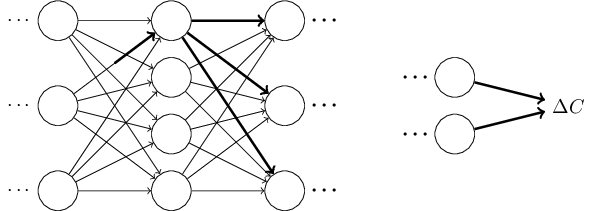
\includegraphics[width=.60\textwidth]{backProbError.png}
  \caption{The path how a change in one weight influences the loss function.\cite{Nielsen2015}
}\label{fig:backProbError}
\end{figure}
Equation \ref{eq:deltaC} shows how $\Delta C$ is related to $\Delta w^l_{jk}$
\begin{equation}\label{eq:deltaC}
\Delta C \approx \frac{\partial C}{\partial w^l_{jk}} \Delta w^l_{jk}
\end{equation}
where $l, j, k$ depict the $l^{th}$ layer, the $j^{th}$ neuron and the $k^{th}$ weight respectively.
The change invoked on the activation function is given by
\begin{equation}\label{eq:deltaA}
\Delta a^l_j \approx \frac{\partial a^l_j}{\partial w^l_{jk}} \Delta w^l_{jk}
\end{equation}
This change influences the next activation function as described in Equation \ref{eq:deltaA+}
\begin{equation}\label{eq:deltaA+}
\Delta a^{l+1}_q \approx \frac{\partial a^{l+1}_q }{\partial  a^l_j} \Delta  a^l_j
\end{equation}
Substituting from Equation \ref{eq:deltaA} leads to 
\begin{equation}\label{eq:deltaA++}
\Delta a^{l+1}_q \approx \frac{\partial a^{l+1}_q }{\partial  a^l_j}\frac{\partial a^l_j}{\partial w^l_{jk}} \Delta w^l_{jk} 
\end{equation}
The change in $\Delta a^{l+1}_q $ again causes change in the following layers. 
Imagining a path of activation $ a^l_j ,  a^{l+1}_q, \cdots, a^{L-1}_n, a^{L}_m$ the change in $\Delta C$ is given by
\begin{equation}\label{eq:deltaCfull}
\Delta C \approx \frac{\partial C}{\partial a^{L}_{m}} \frac{\partial a^{L}_{m}}{\partial a^{L-1}_{n}} \frac{\partial a^{L-1}_{n}}{\partial a^{L-2}_{p}} \cdots \frac{\partial a^{l+1}_{q}}{\partial a^{l}_{j}} \frac{\partial a^{l}_{j}}{\partial w^{l}_{jk}} \Delta  w^{l}_{jk}
\end{equation}
This only considers one path through the neural network, but to compute the gradient with respect to a certain weight all possible paths must be considered.
Equation \ref{eq:gradWRTw} shows how the change in one weight influences the loss function by the influence to all connected neurons and their respective activation functions.
\begin{equation}\label{eq:gradWRTw}
\frac{\partial C}{\partial w^{l}_{jk}} = \sum_{mnp \cdots q} \frac{\partial C}{\partial a^{L}_{m}} \frac{\partial a^{L}_{m}}{\partial a^{L-1}_{n}} \frac{\partial a^{L-1}_{n}}{\partial a^{L-2}_{p}} \cdots \frac{\partial a^{l+1}_{q}}{\partial a^{l}_{j}} \frac{\partial a^{l}_{j}}{\partial w^{l}_{jk}}
\end{equation}
This very intuitively shows how an error needs to propagated back through the network to optimize the loss by applying small changes to the weights with the use of gradient descent.
As explained earlier this technique relies highly on the loss surfaces and respectively the gradients. 
As the error propagates back through the NN by multiplication of the gradients it is easy to see that values can vanish if the multiplicators are rather small and will be multiplied often. 
This is called the \emph{vanishing gradient}
The opposite (\emph{exploding gradient}) happens if the gradient values are constantly bigger than $1$. 
This problem is easy to handle if values are limited by $1$.
In modern Frameworks like TensorFlow and Theano automatic differentiation(AD) is used which makes it easy to setup experimental DNNs without the need to explicitly differentiating activation and loss functions.\cite{ValdenegroToro2019DeepNN}


\subsection{Loss Function}\label{ssec:lossFunc}
As already seen in the preceding sections the \emph{Loss Function}(sometimes also referred to as \emph{Cost Function}) is an essential part in the Learning Process.
The loss function is a scalar function which reflects how "good" or "bad" predictions are in comparison with the \emph{Ground Truth}.
What "good" or "bad" means can strongly depend on the domain of the problem.
For different problems different loss functions are needed. 
In the following the four most important loss functions and it's applications will be discussed.
\paragraph{Mean Squared Error (MSE)}
The MSE is a very intuitive loss function which is defined by Equation \ref{eq:mse}.
\begin{equation}\label{eq:mse}
MSE(\hat{y}, y) = \frac{1}{n} \sum_{i = 0}^{n}(\hat{y}_i - y_i)^2
\end{equation}
The error between the prediction $\hat{y}$ and the label $y$ is defined by their difference, while the squaring helps producing only positive values. The MSE is also called $L_2$ loss because it is defined using the $L_2$ norm.
The MSE is typically used for regression tasks.
One problem with the MSE is that due to the square term,
large errors are penalized more heavily than smaller ones. This
produces a practical problem where using the MSE loss might lead
the convergence of the output to a mean of the ground truth values
instead of predicting values close to them.\cite{ValdenegroToro2019DeepNN}
\paragraph{Mean Absolute Error (MAE)}
The MAE or $L_1$ loss can get around this problem because it is given by
\begin{equation}
MAE(\hat{y}, y) = \frac{1}{n} \sum_{i = 0}^{n}|\hat{y}_i - y_i|
\end{equation}
The absolute error leads to the drawback that the MAE is not differentiable in it's origin.
The L1 loss can recover the median
of the targets, in contrast to the mean recovered by the L2 loss.\cite{ValdenegroToro2019DeepNN}
The MAE is like the MSE generally applied for regression tasks
\paragraph{Categorical Cross-Entropy (CCE)}
In classification a probability value $\hat{y}^c$ is given for every class $c$ in the classification domain $C$. 
CCE has proven to produce smoother loss surfaces for classification tasks and does not have the outlier weighting problem the MSE faces.
The CCE is defined as
\begin{equation}\label{eq:cce}
CCE(\hat{y}, y) = - \sum^n_{i = 0} \sum^C_{c = 0} y_i^c \mathrm{log} \hat{y}_i^c
\end{equation} 


\paragraph{Binary Cross-Entropy (BCE)}
For binary classification $\hat{y}$ is the probability of the positive class and Equation \ref{eq:cce} unfolds to 
\begin{equation}
BCE(\hat{y}, y) = - \sum^n_{i = 0} \left[ y_i \mathrm{log} \hat{y}_i + (1-y_i) \mathrm{log}(1-\hat{y}_i) \right]
\end{equation}

\subsection{Hyper-parameter Tuning}\label{ssec:hyperP}
What is the difference between parameters and \emph{hyper-parameters}?
The parameters are learned by the algorithm in the learning process and for ANNs they are normally referred to as the \emph{weights} of the ANN, whileas the \emph{hyper-parameters} will not be learned but need to decided by the human designer of the ANN or any other learning algorithm.
In the case of an ANN the hyper-parameters are for example the number of layers, the number of artificial neurons per layer, the type of neurons, the type of connection between layers, the learning rate for the optimizer, the batch size and the number of epochs to train the model.
The hyper-parameters basically decide if the model will be able to learn the implicit mapping given in the data.
\paragraph{Model complexity}
The model complexity is given by the number of parameters the learning algorithm needs to learn.
A model with too high complexity is prone to overfitting, while a model with too low complexity is prone to underfitting.
The goal is to find a model complexity, that perform very well on the training data but also generalizes to unseen data.
To achieve this kind of robustness \emph{regularization techniques} exist for basically any learning algorithm (see Section \ref{ssec:regularization}). 
\paragraph{Learning Rate}
As depicted in Figure \ref{fig:lr} the learning rate is very important for convergence. 
If the learning rate is to high the optimization process will fail by not finding the minimum but diverge around it.
On the other hand if the learning rate is to low convergence will happen but happens very slow. 
A good learning rate is crucial for fast convergence.
Typically learning rates in the range $[0, 1]$ are chosen, but it is common to take small values as negative power of 10 like $\alpha = [0.1, 0.01, 0.001]$.
The learning rate does not need to be static over the learning process and can be adjusted dynamically.
The typical
method is to decrease the LR by a factor after a plateau of the loss
curve has been detected, which potentially could allow the loss
to decrease further. \cite{ValdenegroToro2019DeepNN}
This can be imagined as throwing a ball in a loss surface which will roll in the lowest hollow. If it stops the ball will be changed for a smaller ball which will roll even lower in this hollow.
\paragraph{Batch Size}
As described in Section \ref{ssec:gradientDescent} the \emph{batch size} decides how many samples will be taken into account for one update of the MGD and that it is normally chosen as a power of two to efficiently use memory.
Bigger batches make a better approximation of the true gradient and decrease computation time but increase the memory needed for the computation.
The biggest possible batch size really depends on the model complexity but should be chosen to the maximum possible with given memory configurations.
\paragraph{Number of Epochs}
The \emph{number of epochs} decides about the length of training.
If this hyper-parameter is chosen too small the loss may have not converged at this time.
If it chosen to big training takes longer than needed and the risk of overfitting arises if no regularization means are used.
A way of getting a good compromise in an automated way is the early stopping criterion, which can monitor the validation loss or validation accuracy and stop if they are no longer decreasing or increasing respectively. 
This makes it possible to only set a reasonable minimum for the number of epochs.


\subsection{Over- / Underfitting}\label{ssec:overfitting}
The problem of \emph{overfitting} and \emph{underfitting} is as old as learning in general.
Overfitting happens if the model adjust too strong to the training data and therefore is no longer able to generalize to new data.
On the other hand underfitting is the complete opposite where the model generalizes to much so it can not properly map the real distribution of the data.
An intuitive example would be two students who learn for a test in a Chinese class but both aren't able to understand the language.
The test is multiple choice and they have some example tests for learning.

\textbf{Student A (the \emph{underfitter})} just looks at all the answers and realizes that most of the answers are in checkbox 2, so he decides to just tick checkbox two on every question. This leads to a bad score even in the example tests handed out for learning.

\textbf{Student B (the \emph{overfitter})} learns every question and the corresponding answers by heart which results in a perfect score in the example tests handed out for learning. If the final test includes the exact questions from the examples student B got lucky but if the questions and answers change their wording student B will perform poorly on the test. 

From a data perspective Figure \ref{fig:underfitting} - \ref{fig:overfitting} show how a linear regression underfitts with a polynomial degree of 0, while choosing a polynomial degree of 8 leads to overfitting.

\begin{figure}
\centering
  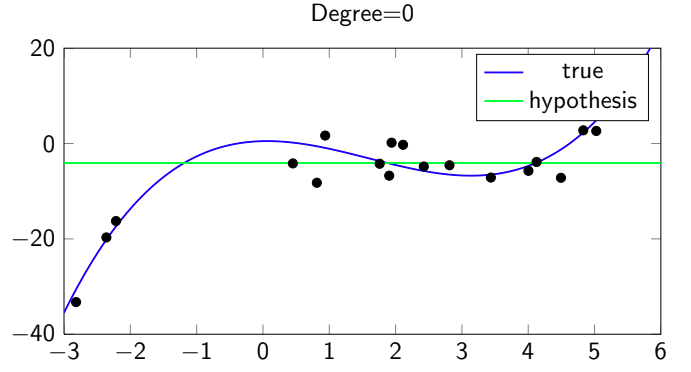
\includegraphics[width=.60\textwidth]{underfitting.png}
  \caption{The chosen model performs poorly even on the training data\cite{LVDFKI}
}\label{fig:underfitting}
\end{figure}

 \begin{figure}
\centering
  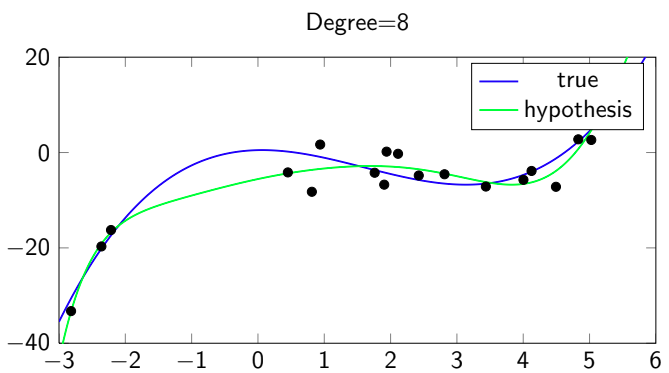
\includegraphics[width=.60\textwidth]{overfitting.png}
  \caption{The model performs very well on the training data but does not model the true function which is a polynominal with degree 3. \cite{LVDFKI}
}\label{fig:overfitting}
\end{figure}


\subsection{Regularization}\label{ssec:regularization}
Generally speaking regularization is a technique to prevent overfitting.
For the linear regression example in Figure \ref{fig:underfitting} - \ref{fig:overfitting} Tikhovnov regularization can be applied which penalizes large weights that are not supported by evidence from the data. This reduces the influence of higher polynomials(this variant of linear regression is called \emph{ridge regression}).
Although it is possible to apply Tikhovnov regularization(also called $L_2$ regularization) deep learning techniques like \emph{Dropout} and \emph{Batch Normalization} have proven to work very well while being easy to implement.
\paragraph{Dropout}
Dropout randomly removes neurons from the network for each iteration. 
This simple step simulates training a large number of NNs with slightly different model structures in parallel.
Figure \ref{fig:dropout} depicts one possible randomly chosen model structure.

 \begin{figure}
\centering
  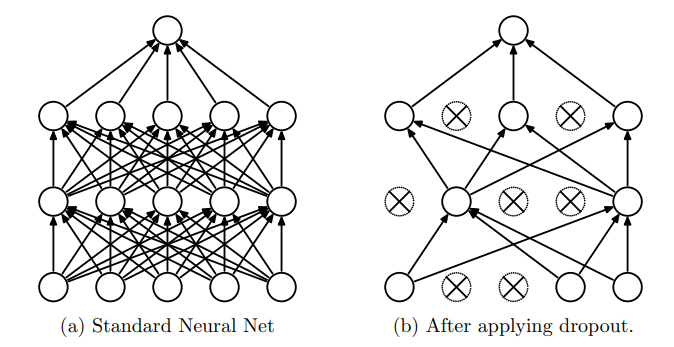
\includegraphics[width=.60\textwidth]{dropout.png}
  \caption{Dropout Neural Net Model. \textbf{Left:} A standard neural net with 2 hidden layers. \textbf{Right:}
An example of a thinned net produced by applying dropout to the network on the left.
Crossed units have been dropped. \cite{JMLR:v15:srivastava14a}
}\label{fig:dropout}
\end{figure}

Srivastava et al. figured that \emph{units may change in a way that they fix up the mistakes of the other units. This may lead to complex co-adaptations. This in turn leads to overfitting because these co-adaptations do not generalize to unseen data.}\cite{JMLR:v15:srivastava14a}
The suggested solution to break up the co-adaptions was to introduce noise in the form of a mask $\mathbf{m}$ of length n.
Every entry in this mask is either $0$ or $1$ with a probability $p$ to be $1$.
The \emph{dropout layer} can be imagined as a layer that cuts some connections (multiplication with $0$) and lets some of the connections through (multiplication with $1$). 
This mask is ordered new in every iteration, meaning the neurons that will be cut off will change in every iteration.
While neurons will be dropped during training this is not the case for inference or testing. To account the for the absence of $(1-p)\%$ of the neurons during the training all activation functions will be multiplied by $p$.
Srivastava et al. showed in Figure \ref{fig:dropoutResults} that using dropout layers invokes an increase in the robustness of several DNNs and therefore decreases the classification error of those DNNs drastically.

 \begin{figure}
\centering
  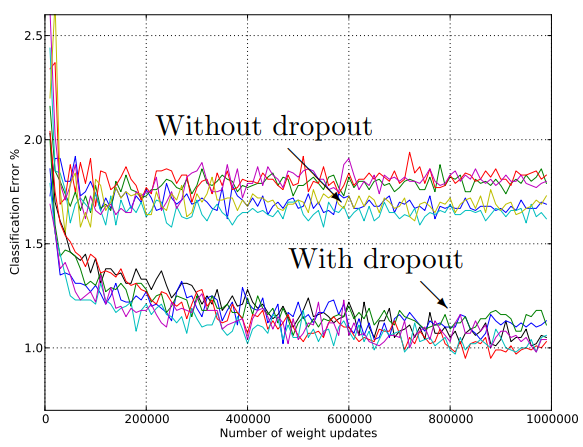
\includegraphics[width=.60\textwidth]{dropoutResults.png}
  \caption{Test error for different architectures
with and without dropout. The networks have 2 to 4 hidden layers each
with 1024 to 2048 units. \cite{JMLR:v15:srivastava14a}
}\label{fig:dropoutResults}
\end{figure}

\paragraph{Batch Normalization}
%die verteilung des inputs eines layers ändert sich andaurnd während des trainings, weil die gewichte der vorherigen layer angepasst werden. Das verlangsamt das training und wird s internal covariate shif gennannt. Jeder eingehende batch wird normalisiert, was diesen Effekt veringert und dadurch Lernen schneller machen kann. Liegt wahrscheinlich auch daran, dass die loss surface smoother ist.
Batch normalization is a technique developed to enhance the training speed but has the nice side effect of regularizing quite well.
The general idea Sergey Ioffe et al. where pursuing in \cite{ioffe2015batch} was to reduce \emph{internal covariate
shift}. \emph{internal covariate
shift} is described as the phenomenon that the distribution of each layer's input is changing during training due to the adaption of weights.
\emph{ The
intuition for Batch Normalization is that drastic internal covariate
shift is prejudicial for neural network training, as it is more likely to saturate non-linearities, and unstable activation distributions
will need more training iterations to converge successfully. Both
situations causes slow training convergence.}\cite{ValdenegroToro2019DeepNN}
The normalization is performed component-wise on the features, so that features have a mean of $0$ and a standard deviation of $1$.
The mean of a batch is given by
\begin{equation}
\mu_B = \frac{1}{|B|} \sum_{i=0}^m x_i
\end{equation}
and the variance of the batch is given by
\begin{equation}
\sigma^2_B = \frac{1}{|B|} \sum_{i=0}^m (x_i - \mu_B )^2
\end{equation}
The normalized features of the batch are then defined as
\begin{equation}
\hat{x}_i = \frac{x_i - \mu_B}{\sqrt{\sigma^2_B + \epsilon}}
\end{equation}
where the batch $B = {x_0, \cdots, x_m}$,  $|B|$ is the size of the batch and $\epsilon = 0.001$ is a very small constant to prevent division by zero.
The scaled shift is applied by
\begin{equation}
y_i = \gamma \hat{x}_i + \beta
\end{equation}
where $\gamma$ and $\beta$ are parameters that need to learned.
Batch normalization is a very stable technique with basically no drawbacks, that is why it is used by most modern NN architectures (for example ResNet, GoogleNet and DenseNet use it).
Shibani Santurkar et al. show in \cite{2018arXiv180511604S} that batch normalization smoothes the loss surface and therefore achieves the regularization effect.

\subsection{Convolutional Layers}\label{ssec:Conv}
A convolutional layer is a layers in a NN in which the artificial neuron described earlier are replaced with a filter(sometime also referred to as kernel).
The \emph{convolutional layer} has its name because these filters perform convolution on the input data.
\subsubsection{Convolution}\label{ssec:convolution}
Mathematically speaking \emph{convolution} is expressing how the shape of one function modifies the other and is defined by
\begin{equation}\label{eq:convolution}
(f * g) = \int_{\mathbb{R}^n} f(\tau)g(x-\tau)\mathrm{d}\tau
\end{equation}
Because Equation \ref{eq:convolution} may not be very intuitive the following example will show convolution on an image, because that is what it is used for in CNNs.
An image can be imagined as a 2-dimensional discrete function $f: \mathbb{Z}^{W \times H}  \rightarrow \mathbb{Z}^Z$ which maps every $(x,y)$ position to a pixel value $z$.
Where $W$ denotes the \emph{width}, $H$ the \emph{height} and $Z$ the pixel value.
If a grayscale image is considered $z \in [0, 255]$(the range $[0, 255]$ is internally often represented as the range $[0, 1]$).
Now the second function is needed and this is the filter. 
A filter $\omega: \mathbb{Z}^{M \times N}  \rightarrow \mathbb{R}$ is a 2-dimensional discrete function which describes how each pixel will be influenced by its neighboring pixels. Although filters can have different dimensions for $N$ and $M$ they are normally designed as being quadratic.
Figure \ref{fig:filter} shows the results of convolving a filter designed to detect edges on a small sample image.
\begin{figure}
\centering
  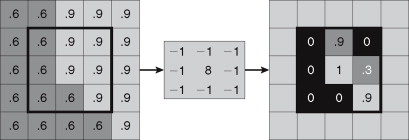
\includegraphics[width=.80\textwidth]{edgeDetection.jpg}
  \caption{3 x 3 filter for edge detection applied on small sample image \cite{BRINKMANN200893}
}\label{fig:filter}
\end{figure}
Applying the filter is done by calculating a weighted average for every pixel in the image therefore the filter is shifted over the whole image.
This is defined by
\begin{equation}
g(x,y) = \omega * f(x,y) = \sum_{s=\left \lceil-M/2 \right \rceil}^M \sum_{s=\left \lceil-N/2 \right \rceil}^N \omega(s, t)f(x-s, y-t)
\end{equation}\label{eq:filter}
The definition in Equation \ref{eq:filter} assumes that the summation point for the filter is in $\omega(0,0)$ and the positions within the filter range from $[\left \lceil-M/2 \right \rceil, \left \lfloor M/2 \right \rfloor]$ and $[\left \lceil-N/2 \right \rceil, \left \lfloor N/2 \right \rfloor]$ respectively, which also implies that the \emph{width} $M$ and the \emph{height} $N$ of the filter must be odd values.
For the given example in Figure \ref{fig:filter} starting from the upper left corner this leads to $g(1,1) = 0.6 * (-1) + 0.6 * (-1) + 0.9 * (-1) + 0.6 * (-1) + 0.6 * (8) + 0.9 * (-1) + 0.6 * (-1) + 0.6 * (-1) + 0.9 * (-1) = -0.9 $, which will be clipped to the domain of $[0,1]$ resulting in $g(1,1) = 0$.
Then the filter will be shifted one step to the right which leads to $g(2,1) = 0.6 * (-1) + 0.9 * (-1) + 0.9 * (-1) + 0.6 * (-1) + 0.9 * (8) + 0.9 * (-1) + 0.6 * (-1) + 0.9 * (-1) + 0.9 * (-1) = 0.9$. This is performed for the whole image until it leads to the output depicted in Figure \ref{fig:filter}.
Filters with different weights have different functions.
While the filter in the given example is used for edge detection different configurations can be used for blurring, sharpening and many other applications. 
A convolutional layers is constructed from multiple filters and the output of it is given by

\begin{equation}
\mathbf{y}= f(\mathbf{x} * \mathbf{F} + b)
\end{equation},
where $\mathbf{x}$ is the input image, $\mathbf{F}$ is the filter, $b$ is the bias and $f$ is the activation function.
For every filter in the layer a new image is created. 
These images are called \emph{convolutional feature map}, because they represent specific visual features extracted by the filter(for example edges).
The filter weights and biases in a convolutional layer are not set like in the edge detection example, but are learned while performing gradient descent.
\subsubsection{Convolutional Neural Networks (CNNs)}\label{ssec:convNets}
As described in Section \ref{ssec:Conv} convolutional filters can be trained to detect specific features in images.
These features have the big advantage that they can be calculated position independent.
If processing an image with a NN with classical neurons every neuron would be connected to a pixel and therefore could only make sense for that specific pixel.
For image classification this would mean the classification of a specific object in an image can only be made if the object will always be in the same place. This is not very helpful.
As explained filters go over the whole image and calculate a new image with respect to a certain feature.
A CNN which classifies letters would most certainly learn filters for horizontal, vertical and different diagonal edges and some more for different types of corners in its first layer.
The followings layer would learn filters as some combination of those. An "A" for example consists of two diagonal lines and a horizontal line and it does not matter where in the image the structure appears it only matters that the features(lines and edges in this case) are in the same constellation.
If the aim is to classify more complex structures it is important to account the hierarchy of features.
The combination of features like edges and corners will take place on a bigger scale.
Therefore either the filters on the following layer need to be bigger or the resulting feature map needs to be down sampled.
The latter is called \emph{Pooling} and is for reasons of performance and memory efficiency the preferred solution.
The parameters the CNN would need to learn with enlarging the filters would grow exponentially.
On top of the convolutional layers a dense layer is needed to make the classification. 
With this being connected to a very big convolutional feature map resulting from a CNN without pooling the dense layer becomes very big and is therefore prone to overfitting.
Pooling can be performed using a $M \times M$ grid and shifting it over the feature map with a step size of $M$. For every step the maximum(for Max-Pooling) or the average(for Average-Pooling) is calculated. 
These new values represent the the down sampled feature map. 
The down sampling is performed by the rate $M^{-2}$.

CNNs have proven to be state of the art in image classification tasks since in 2012 the AlexNet was winning the Large Scale Visual Recognition Challenge (ILSVRC) \cite{ILSVRC} competition with a top-5 test error rate of 15.3\%,
compared to 26.2\% achieved by the second-best entry.\cite{NIPS2012_4824}
So today CNNs have become the standard for NNs and images but they are also used for sound related learning tasks like voice recognition or speaker identification.
This is the case because a sound signal can be fully represented as an image of a sound wave.
CNNs perform good on data where features close to each other also have a close relation between each other.
Images obviously comply with this rule, because if all pixels of an image would be shuffled all information would be lost.
\subsection{Recurrent Layers}
All NNs described before are \emph{feedforward neural networks}.
That means that information is passing the network only from input towards output.
Feedforward NNs are working very well for a lot of problem settings but they are not able to save an internal state.
The human brain in contrast processes information in sequence and produces an internal model of prior processed information, which continuously changes by the influence of new input.
Reading for example takes as input one word at a time and produces an internal model of the text.
In the "real world" everything is attached to the time and therefore this applies to every aspect of learning in the human brain. 
In data science it is a common practice to only consider data at a specific point in time, which makes it possible to use feedforward NNs for a wide variety of tasks.
But if a temporal relation needs to be modeled Recurrent Neural Networks(RNNs) are the approach to model these time dependent tasks.

Figure \ref{fig:RNN} shows that RNNs use loops to use the output of a recurrent layer as part of its input. 
This behavior is defined by
\begin{equation}
\mathbf{h}^{(t)} = f(\mathbf{h}^{(t-1)}, \mathbf{x}^{(t)}; \mathbf{\theta})  
\end{equation}\label{eq:RNN}
where $\mathbf{h}^{(t)}$ is the state at time $t$ and $f$ a function that calculates the state $\mathbf{h}^{(t)}$ from the state $\mathbf{h}^{(t-1)}$ at time $t-1$ and the input $\mathbf{x}^{(t)}$ at time $t$ and a given set of parameters $\theta$.
\begin{figure}
\centering
  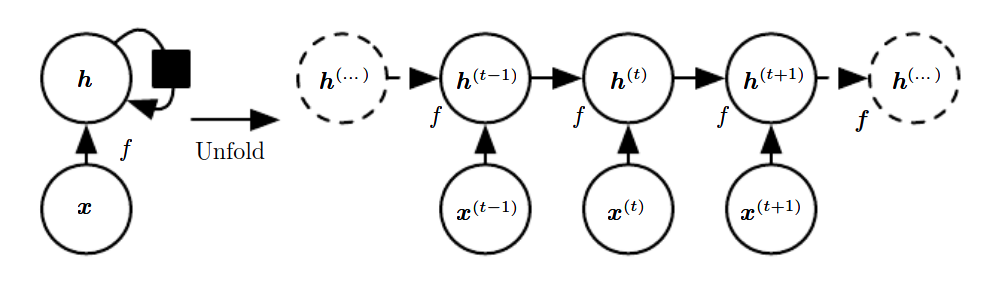
\includegraphics[width=.75\textwidth]{RNN.png}
  \caption{A recurrent network with no outputs. This recurrent network just processes information from the input $\mathbf{x}$ by incorporating it into the state $\mathbf{h}$ that is passed forward through time. (Left) Circuit diagram. The black square indicates a delay of a single timestep. (Right) The same network seen as an unfolded computational graph, where each node is now associated with one particular time instance. \cite{Goodfellow-et-al-2016}
}\label{fig:RNN}
\end{figure}
Figure \ref{fig:RNNLearn} shows how learning is applied to the given structure with labels $\mathbf{y}$, outputs $\mathbf{o}$ and a loss function $L$.
\begin{figure}
\centering
  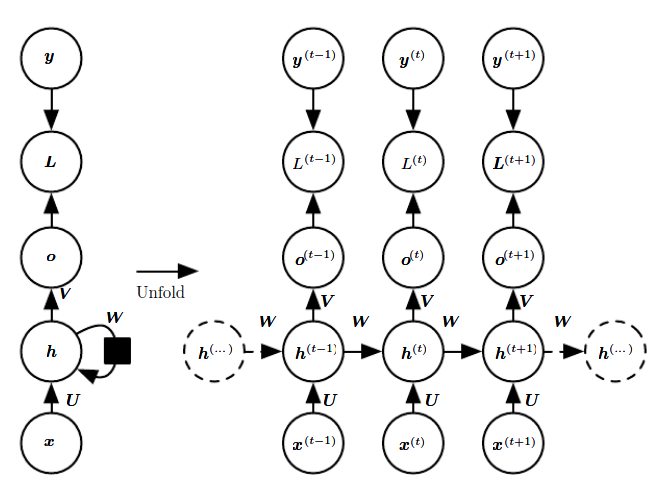
\includegraphics[width=.75\textwidth]{RNNLearn.png}
  \caption{The computational graph to compute the training loss of a  recurrent 
  network that maps an input sequence of 
$\mathbf{x}$ 
 values to a corresponding sequence of output $\mathbf{o}$ values. A loss $L$ measures how far each $\mathbf{o}$ is from the corresponding training target $\mathbf{y}$. When using softmax outputs, we assume $\mathbf{o}$ is the unnormalized log probabilities. The loss $L$ internally computes $\hat{y}=softmax(\mathbf{o})$ and compares this to the target $\mathbf{y}$. The RNN has input to hidden connections parametrized by a weight matrix $\mathbf{U}$, hidden-to-hidden recurrent connectionsparametrized by a weight matrix $\mathbf{W}$, and hidden-to-output connections parametrizedby a weight matrix $\mathbf{V}$.(Left) The RNN and its loss drawn with recurrent connections. (Right) The same seen as a time-unfolded computational graph, where each node is now associated with one particular time instance. \cite{Goodfellow-et-al-2016}
}\label{fig:RNNLearn}
\end{figure}


\subsection{Long Short-Term Memory (LSTM)}\label{ssec:LSTM}
The classical RNN structure suffers from the problem of the vanishing gradient.
Sepp Hochreiter and Jürgen Schmidhuber proposed a solution to that problem in \cite{LSTM}.
The proposed architecture is called Long Short-Term Memory(LSTM) and introduces a short-term memory that is able to learn on time series of over 1000 discrete timesteps.
Figure \ref{fig:LSTMFig} shows that the LSTM comes with \emph{input, output, forget gate} to control input and output of the cell.

\begin{figure}
\centering
  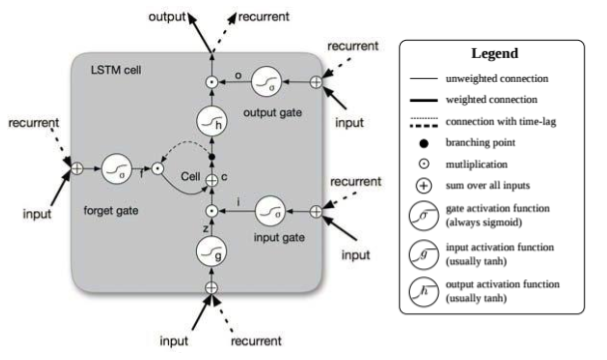
\includegraphics[width=.90\textwidth]{LSTMFig.png}
  \caption{Detailed schematic of a Long Short-Term Memory cell \cite{LSTMFig}
}\label{fig:LSTMFig}
\end{figure}

These gates have very descriptive names.
The input gate controls if(or better when) input is taken into consideration to update the internal state.
The output gates controls the output in the same way, whileas the forget gate controls when the internal state should be reset and when it should be sustained.
If the forget gate sustains the state of the cell the state will always be added to the activated and gated input in the next step.
Hochreiter and Schmidhuber called this internal time shifted addition the \emph{Constant Error Carrousels}(CEC).
The addition in the CEC prevents the problem of the vanishing gradient.
While feed forward networks can only be used to make a one to one prediction, LSTMs(and other RNN structures) can be used for different types of predictions.
\paragraph{one to many} predictions take a single input and produce a sequence of outputs.
This can find application in captions for images where the caption can be a sentence of a variable length.
In this case the output gate controls how the sequence of words will be shaped. 
For example an image showing a dog chasing a ball should be described as "Dog chasing ball" but not as "Ball chasing dog" although the same words are used.
The weights of the output gates of the LSTM layer in this case implicitly know about the structure of a sentence and the meaning of the words and how they make sense.
\paragraph{many to one} prediction work with a sequence as input and produce a single output.
This is how predictions for the VVAD are working. The NN takes a sequence of features(face images, lip images, facial features or lip features) as input and predicts if this sequence is a positive \emph{speaking} or a negative \emph{not speaking} sample.
Here the input gate learns which timesteps of the input data should be considered to update the internal state.
\paragraph{many to many} or \emph{sequence to sequence} predictions use a sequence as input data and produce a sequence as output. 
This can be used to extend the image caption example to video captions. Another application is speech recognition where voice(a sequence of frequencies) is taken as input to predict a sequence of words.

%TODO feature extraction am besten in convNets kurz erklären

%TODO Metrics https://towardsdatascience.com/metrics-to-evaluate-your-machine-learning-algorithm-f10ba6e38234 (Bonus)



 
%TODO data augemtation(Bonus)

